% Régresseurs fortement corrélés : corr(b1,b2) = -0,9, écarts-types unitaires,
% b̂ = (1,5 ; 1,4). Ellipse jointe à 95 % : (b-b̂)'V[b̂]^{-1}(b-b̂) = 5,991.
% Demi-axes 3,374 (à -45°) et 0,774 ; demi-largeur de la boîte englobante 2,448,
% à comparer aux 1,96 des intervalles individuels.
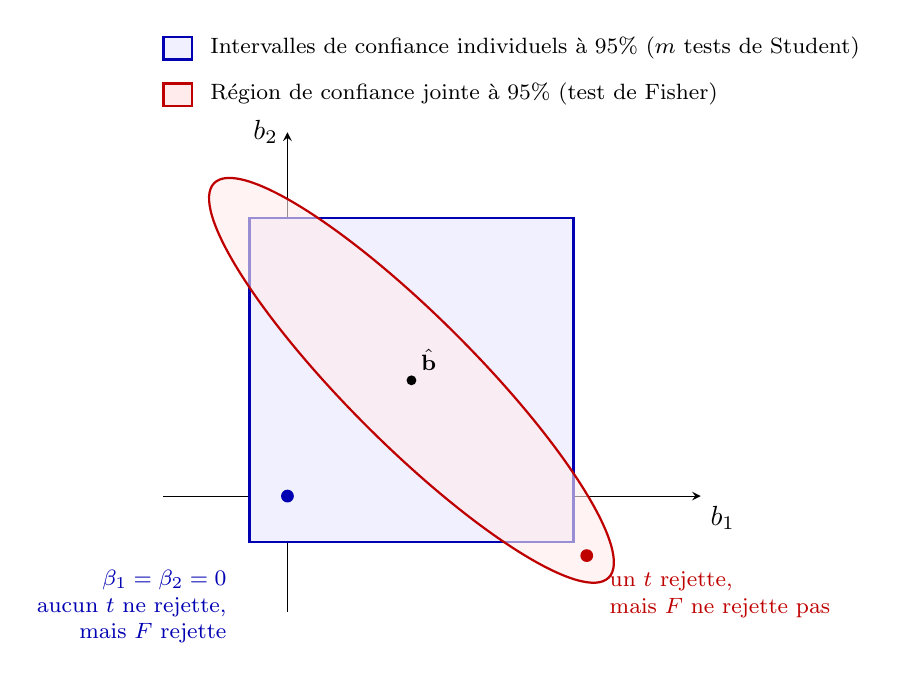
\begin{tikzpicture}[>=stealth, scale=1.05]

  % Légende, au-dessus du graphique pour ne rien recouvrir.
  \draw[thick, blue!70!black, fill=blue!6] (-1.5,5.28) rectangle (-1.15,5.55);
  \node[anchor=west, font=\footnotesize] at (-1.05,5.42)
       {Intervalles de confiance individuels à $95\%$ ($m$ tests de Student)};
  \draw[thick, red!75!black, fill=red!8] (-1.5,4.72) rectangle (-1.15,4.99);
  \node[anchor=west, font=\footnotesize] at (-1.05,4.86)
       {Région de confiance jointe à $95\%$ (test de Fisher)};

  \draw[->] (-1.5,0) -- (5.0,0) node[below right] {$b_1$};
  \draw[->] (0,-1.4) -- (0,4.4) node[left] {$b_2$};

  % Rectangle : produit des deux intervalles de confiance individuels.
  \draw[thick, blue!70!black, fill=blue!6] (-0.46,-0.56) rectangle (3.46,3.36);

  % Ellipse : région de confiance jointe.
  \draw[thick, red!75!black, fill=red!8, fill opacity=.6,
        rotate around={-45:(1.5,1.4)}] (1.5,1.4) ellipse [x radius=3.374, y radius=0.774];

  % L'estimateur.
  \fill (1.5,1.4) circle (1.7pt) node[above right, font=\footnotesize] {$\hat{\mathbf b}$};

  % Cas 1 : l'origine. Dans le rectangle, hors de l'ellipse.
  \fill[blue!70!black] (0,0) circle (2.2pt);
  \node[anchor=north east, font=\footnotesize, blue!70!black, align=right] at (-0.62,-0.78)
       {$\beta_1=\beta_2=0$\\ aucun $t$ ne rejette,\\ mais $F$ rejette};

  % Cas 2 : hors du rectangle, dans l'ellipse.
  \fill[red!75!black] (3.62,-0.72) circle (2.2pt);
  \node[anchor=north west, font=\footnotesize, red!75!black, align=left] at (3.78,-0.80)
       {un $t$ rejette,\\ mais $F$ ne rejette pas};

\end{tikzpicture}
